\section{同调流形}
\sourcepage{451}
本节定义同调流形，并研究它们的一些局部性质。同调流形包含所有拓扑流形，因此是一类广泛而重要的空间。可三角剖分的同调流形将是各种对偶定理中的基本研究对象。

为方便起见，本节直接讨论相对同调流形，尽管直到第 8.10 节才会真正证明相对情形的对偶定理。

先约定一种记号上的简化。我们所研究的空间都可三角剖分。如果 $X$ 已配有一个特定的三角剖分，常常不在记号上区分空间与剖分它的复形。例如可以说空间 $X$ 的一个点，也可以说复形 $X$ 的一个单形，具体含义由上下文说明。

\entry{定义}{8.3.1}拓扑偶 $(X,A)$ 称为\emph{相对同调 $n$ 维流形}，如果对每个 $x\in X\setminus A$，局部同调群满足
\[
H_i(X,X\setminus\{x\})\cong
\begin{cases}\Z,&i=n,\\0,&i\ne n.\end{cases}
\]
当 $A$ 为空时，简称 $X$ 为\emph{同调 $n$ 维流形}。

若 $M$ 是带边界的 $n$ 维流形，则 $(M,\Bd M)$ 是相对同调 $n$ 维流形（见第 4.8 节）。更一般地，只要 $X\setminus A$ 是 $n$ 维流形，$(X,A)$ 就是相对同调 $n$ 维流形。

若 $(X,A)$ 已三角剖分，则 $X$ 的局部同调性质反映在各单形链环的同调群中。下一引理给出这种联系。

\entry{引理}{8.3.2}设 $s$ 是复形 $K$ 的 $k$ 维单形，$\widehat s$ 是其重心，则
\[
H_i(|K|,|K|\setminus\{\widehat s\})\cong
\begin{cases}
\widetilde H_{i-k-1}(\operatorname{Lk}s),&\operatorname{Lk}s\ne\varnothing,\\
H_i(s,\Bd s),&\operatorname{Lk}s=\varnothing.
\end{cases}
\]

\textbf{证明：}若链环为空，$s$ 不是任何更高维单形的面，所以 $\Int s$ 在 $|K|$ 中开。由切除及 $\Bd s$ 是 $s\setminus\{\widehat s\}$ 的形变收缩核，
\[
H_i(|K|,|K|\setminus\{\widehat s\})\cong H_i(s,s\setminus\{\widehat s\})\cong H_i(s,\Bd s).
\]

若链环非空，因重心位于开集 $\operatorname{St}s$ 中，可切除该开集的补集，得到
\[
H_i(|K|,|K|\setminus\{\widehat s\})\cong
H_i(\overline{\operatorname{St}}s,\overline{\operatorname{St}}s\setminus\{\widehat s\}).
\]
\sourcepage{452}
由凸集的基本性质，$|s|=|\widehat s*\Bd s|$，从而由引理 8.2.10，
\[
|\overline{\operatorname{St}}s|=|s*\operatorname{Lk}s|
=|\widehat s*\Bd s*\operatorname{Lk}s|.
\]
按前述约定，$\Bd s$ 为空时等式仍成立。闭星形邻域是以 $\widehat s$ 为顶点的锥，故无环。从锥中删去顶点后，可以形变收缩到底空间（引理 4.8.12）。因此 $|\Bd s*\operatorname{Lk}s|$ 是删去重心后的闭星形邻域的形变收缩核，故
\begin{align*}
H_i(|K|,|K|\setminus\{\widehat s\})
&\cong H_i(\overline{\operatorname{St}}s,\overline{\operatorname{St}}s\setminus\{\widehat s\})\\
&\cong\widetilde H_{i-1}(\overline{\operatorname{St}}s\setminus\{\widehat s\})\\
&\cong\widetilde H_{i-1}(\Bd s*\operatorname{Lk}s)
\cong\widetilde H_{i-k-1}(\operatorname{Lk}s).
\end{align*}
若 $\Bd s$ 为空，则 $k=0$，最后一个同构就是等同；否则由 $\Bd s$ 是拓扑 $(k-1)$ 维球面及定理 8.2.7 得到。\hfill$\square$

\entry{定理}{8.3.3}设 $(X,A)$ 是已三角剖分的相对同调 $n$ 维流形，$s$ 是不属于 $A$ 的 $k$ 维单形。若链环为空，则 $k=n$；若链环非空，则它具有 $(n-k-1)$ 维球面的同调，其中 $n-k-1\ge0$。两种情形下都有 $k\le n$。

\textbf{证明：}重心 $\widehat s\in X\setminus A$，所以该点的局部同调只在 $n$ 维为无限循环群。链环为空时，上一引理给出非零群 $H_n(s,\Bd s)$，所以 $\dim s=n$。链环非空时，其约化同调只在 $n-k-1$ 维为无限循环群，所以 $n-k-1\ge0$。\hfill$\square$

\entry{推论}{8.3.4}设 $(X,A)$ 是已三角剖分的相对同调 $n$ 维流形。
\begin{enumerate}[label=(\alph*)]
\item $X\setminus A$ 的闭包是一些 $n$ 维单形的并。
\item 不属于 $A$ 的每个 $(n-1)$ 维单形恰好是两个 $n$ 维单形的面。
\end{enumerate}

\textbf{证明：}(a) 若 $s\notin A$ 且 $\dim s=k$，则 $k\le n$。若 $k<n$，其链环是同调 $(n-k-1)$ 维球面，因而含有一个 $(n-k-1)$ 维单形 $t$，于是 $s$ 是 $n$ 维单形 $s*t$ 的面。

(b) 对不属于 $A$ 的 $(n-1)$ 维单形 $s$，其链环具有零维球面的同调。由于闭星形邻域维数为 $n$，且等于 $s*\operatorname{Lk}s$，链环必为零维。因此它恰由两个点组成，对应恰好两个 $n$ 维单形。\hfill$\square$

\sourcepage{453}
上述结果说明，已三角剖分的相对同调 $n$ 维流形满足相对伪流形定义的前两个条件（定义 5.4.5）。若 $X\setminus A$ 连通，也满足第三个条件。证明提纲见本节习题；以后也会由对偶定理推导这一事实。

\entry{例}{8.3.5}设 $X$ 是环面 $T$ 与二维球面 $S^2$ 的不交并，$S(X)$ 是其悬挂，$A=\{w_0,w_1\}$ 是两个悬挂点（图 8.3.1）。则 $(S(X),A)$ 是相对同调三维流形，因为 $S(X)\setminus A\approx X\times(-1,1)$ 是三维流形。

子空间偶 $(S(T),A)$ 和 $(S(S^2),A)$ 也都是相对同调三维流形，而且是相对伪三维流形。$S(S^2)$ 是同调三维流形，$S(T)$ 则不是，因为后者中 $w_0$ 的链环是环面，而不是同调二维球面。

\begin{figure}[htbp]\centering
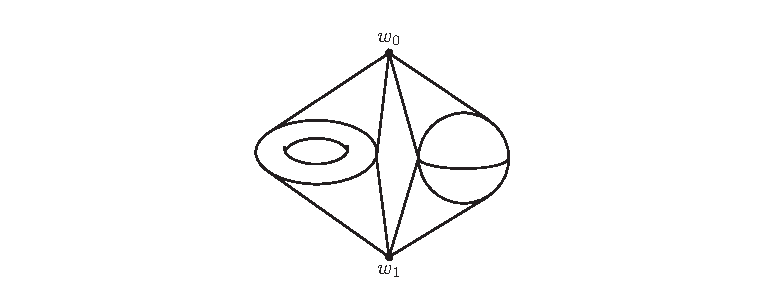
\includegraphics[width=.85\textwidth]{figures/8-3-1.pdf}
\caption*{图 8.3.1}
\end{figure}

\entry{例}{8.3.6}通常所画的流形图形，可能使人猜想：若 $M$ 是已三角剖分的拓扑 $n$ 维流形，则每个 $k$ 维单形的链环都是拓扑 $(n-k-1)$ 维球面。

对通常的二维流形三角剖分，这当然成立：例如边的链环是零维球面，顶点的链环是一维球面。这个猜想长期悬而未决，直到 Robert D. Edwards 和 James W. Cannon 的工作才得到解决（见 [Can79]）。细节较复杂，此处从略。

\entry{例}{8.3.7}确实存在不是拓扑流形的同调 $n$ 维流形。下面概述一种构造，但证明要用到尚未学习的工具。

\sourcepage{454}
所需的基本事实是：存在紧致、已三角剖分的三维流形 $M$，它是同调三维球面，但基本群 $\pi_1(M)$ 不为零。其构造见 [ST80]。原文称其基本群为二十面体群。\translatornote{通常这里的 Poincaré 同调球面的基本群是二元二十面体群；它与普通二十面体旋转群不同。}

取悬挂 $S(M)=M*\{w_0,w_1\}$，则它是同调四维流形。因为除去悬挂点后同胚于四维流形 $M\times(-1,1)$，局部同调条件在其他所有点成立；又因为两个悬挂点的链环均为同调三维球面 $M$，条件在悬挂点也成立。

还需另行证明：在已三角剖分的拓扑 $n$ 维流形中，每个顶点的链环即使不一定同胚于 $(n-1)$ 维球面，也必须具有该球面的同伦型。由于 $\pi_1(M)\ne0$，$M$ 不具有三维球面的同伦型，所以 $S(M)$ 不可能是拓扑四维流形。

以下定理和推论留作习题。

\entry{定理}{8.3.8}若 $(X,A)$ 是已三角剖分的相对同调 $n$ 维流形，且 $X\setminus A$ 连通，则 $(X,A)$ 是相对伪 $n$ 维流形。

\entry{推论}{8.3.9}若 $(X,A)$ 是已三角剖分的相对同调 $n$ 维流形，$s$ 是不属于 $A$ 的单形，则 $\operatorname{Lk}s$ 是有限复形。

\sourcepage{454--455}
\subsection*{习题}
前四题每一题都依赖于前面的习题。
\begin{enumerate}
\item 设 $(X,A)$ 是已三角剖分的拓扑偶。假定对每个不属于 $A$ 的 $k$ 维单形 $s$ 都有：(i) $k\le n$；(ii) 若 $k<n$，则 $H_i(\operatorname{Lk}s)\cong H_i(S^{n-k-1})$。证明 $(X,A)$ 是相对同调 $n$ 维流形。
\item 设 $(X,A)$ 是已三角剖分的相对同调 $n$ 维流形。若 $s\notin A$ 且 $\dim s=k<n$，证明 $\operatorname{Lk}s$ 是同调 $(n-k-1)$ 维流形。〔提示：把链环看作 $X$ 的子复形。对 $t\in\operatorname{Lk}s$，证明
\[\operatorname{Lk}(t,\operatorname{Lk}(s,X))=\operatorname{Lk}(t*s,X).\]〕
\item 证明定理 8.3.8。〔提示：$n=1$ 时显然。假设对小于 $n$ 的维数成立。若存在不属于 $A$ 的 $n$ 维单形序列
\[\sigma=\sigma_0,\sigma_1,\ldots,\sigma_k=\sigma',\]
使每个 $\sigma_i\cap\sigma_{i+1}$ 都是不属于 $A$ 的 $(n-1)$ 维单形，就定义 $\sigma\sim\sigma'$。令 $X_1$ 是一个等价类中元素的并，$X_2$ 是其他等价类中元素的并。若 $s\notin A$ 且 $s\subset X_1\cap X_2$，记 $k=\dim s$，则 $k<n-1$。证明 $\operatorname{Lk}s$ 是伪 $(n-k-1)$ 维流形，进而闭星形邻域中任意两个 $n$ 维单形都等价。〕\translatornote{原文提示中相邻单形下标及“对每个 $i$”有排印错误，此处按相邻关系写出。}
\item 证明推论 8.3.9。〔提示：若 $X$ 是伪 $m$ 维流形且 $H_m(X)\ne0$，则 $X$ 必有限。〕
\item 能否举出第一项空间 $X$ 为圆的相对同调 $n$ 维流形？为什么？
\item 能否举出第一项空间 $X$ 为二维球面的相对同调 $n$ 维流形？为什么？
\end{enumerate}
